\documentclass[12pt]{article}
\usepackage{float}
\restylefloat{table}
\usepackage{graphicx}
\usepackage{rotating}
\usepackage{color}
\usepackage[dvipsnames]{xcolor}
\usepackage{enumitem}
\usepackage{sidecap}
\usepackage[top=15mm, bottom=15mm, left=15mm, right=15mm]{geometry}
\usepackage{multicol}
\usepackage[dvipsnames]{xcolor}
\usepackage{wrapfig}
\usepackage{hyperref}
\usepackage{courier}

\fboxrule=2pt%border thickness

\pagenumbering{gobble}

\setlength\parindent{0pt}

\begin{document}
\title{DEVILS - Observing and On-site Reduction}
\begin{center}

\begin{figure}
\begin{center}
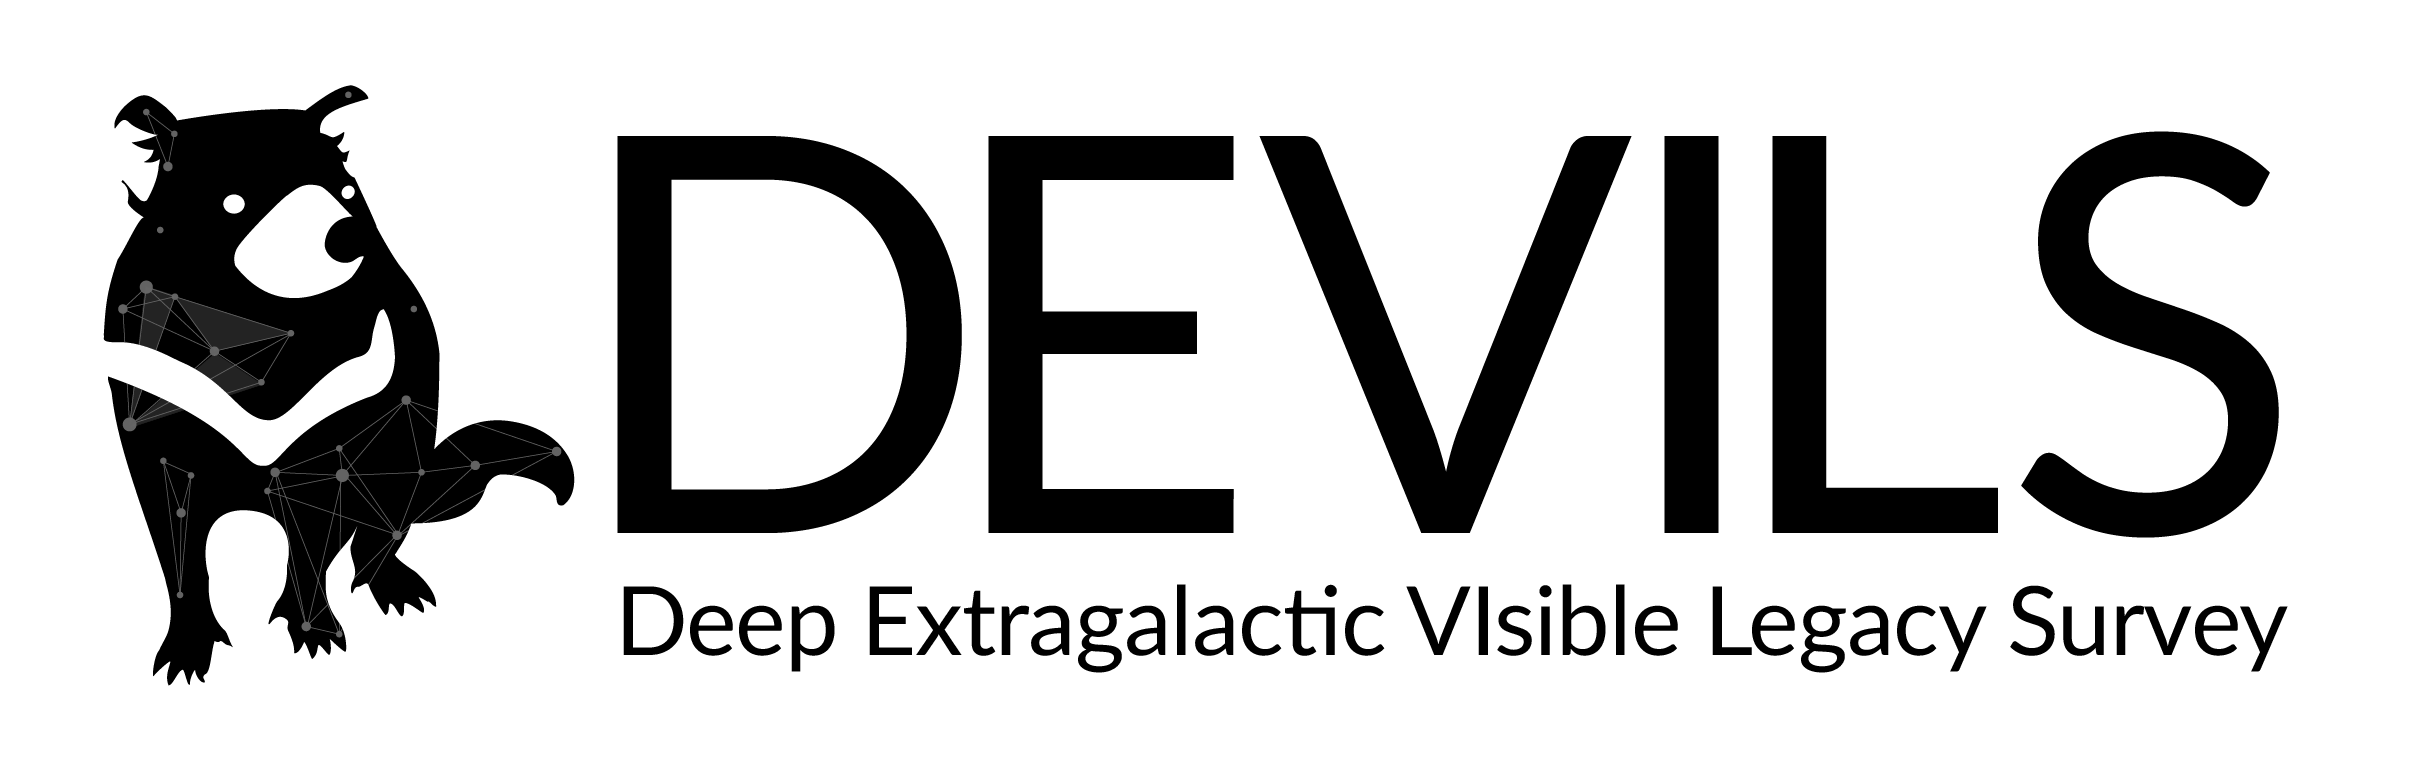
\includegraphics[scale=0.8]{devils-logo_big.png}
\end{center}
\end{figure}

\Huge {\textcolor{PineGreen}{\textbf{Observing and On-site Reduction}}}
\end{center}
\normalsize


\section{The DEVILS directory structure}


On the AAT system at the telescope, there is a DEVILS account. To access this, first get the password from Luke (luke.j.davies@uwa.edu.au). All of the on-site reduction will be done in this workspace.  In the following, `$\sim$' will refer to the DEVILS account?s home directory.\\

\textcolor{PineGreen}{\textbf{NOTE: Please be careful not to delete anything from this space! While we have back-ups, it will take some time to reconstruct things.}}\\

The DEVILS data directories has the following structure:\\

\hspace{5mm} \textbf{data/} 
\vspace{1mm}

\hspace{10mm} \textbf{biases/}
\vspace{1mm}

\hspace{15mm} \textbf{run1\_2017\_12/, ....} 
\vspace{1mm}

\hspace{10mm} \textbf{calibrators/} 
\vspace{1mm}

\hspace{15mm} \textbf{AutoZTemp/} 
\vspace{1mm}

\hspace{15mm} \textbf{filters/} 
\vspace{1mm}

\hspace{15mm} \textbf{GuideStars/}
\vspace{1mm}

\hspace{15mm} \textbf{sensfuncs/}
\vspace{1mm}

\hspace{15mm} \textbf{SkyFibres/}
\vspace{1mm}

\hspace{15mm} \textbf{stdstars/}
\vspace{1mm}

\hspace{10mm} \textbf{darks/} 
\vspace{1mm}

\hspace{15mm} \textbf{run1\_2017\_12/, ....}
\vspace{1mm}

\hspace{10mm} \textbf{idxFiles/} 
\vspace{1mm}

\hspace{10mm} \textbf{logs/} 
\vspace{1mm}

\hspace{10mm} \textbf{observing/} 
\vspace{1mm}

\hspace{15mm} \textbf{D10\_yrPlan2017.png, ....} 
\vspace{1mm}

\hspace{15mm} \textbf{run1\_2017\_12/, ....} 
\vspace{1mm}

\hspace{20mm} \textbf{2017\_12\_18/, ....}
\vspace{1mm}

\hspace{10mm} \textbf{raw/} 
\vspace{1mm}

\hspace{15mm} \textbf{run1\_2017\_12/, ....} 
\vspace{1mm}

\hspace{20mm} \textbf{2017\_12\_18/, ....} 
\vspace{1mm}

\hspace{10mm} \textbf{reduced/}
\vspace{1mm}

\hspace{15mm} \textbf{run1\_2017\_12/, ....} 
\vspace{1mm}

\hspace{20mm} \textbf{2017\_12\_18/, ....} \\


When observing you will add raw data to the \textbf{biases},  \textbf{darks}, and \textbf{raw} data files. The \textbf{observing} directory, will contain information which will help with your observing ($e.g.$ observability plots) and contain text versions of the night logs, which can also be filled in on the wiki here:  \url{https://wiki.devilsurvey.org/mw/index.php?title=Observing}. Further information about these are given below. 

Under each of the \textbf{biases}, \textbf{darks}, \textbf{raw}, \textbf{reduced} and \textbf{observing} directories, you will find a directory for each run with the format \textbf{run1\_YYYY\_MM} ($i.e.$ for run1 in December 2017 - \textbf{run1\_2017\_12}). As biases and darks are common to each run, this is where the raw biases and darks will be placed. 

However, under the \textbf{raw}, \textbf{reduced} and \textbf{observing} directories for each run, there are also sub directories for each observing night, with the format \textbf{YYYY\_MM\_DD} ($i.e.$ the first night of run1 on the 18th of December 2017 can be found in - \textbf{run1\_2017\_12/2017\_12\_18}). Familiarise yourself with this directory structure is it is where all of the DEVILS information and data can be found. If you have used the DEVILS automatic reduction pipeline, TAZ, this is identical to the data structure produced by the \texttt{setUpDir()} function. \\

\textcolor{PineGreen}{\textbf{NOTE: all other directories in this structure you will not need to access as they contain calibrators and/or are used to match the directory structure used by the TAZ (more below)}}

\subsection{Setting up the night directory for your observations}

\textcolor{PineGreen}{\textbf{NOTE: You should not need to do this as it should already be completed by Luke. However, here are instructions for setting up the individual run/night directory structure if it doesn't already exist.}} \\

To set up the directory structure, you simply have to run one shell script, \texttt{setUpDir\_AAT}. This can be found in the \textbf{$\sim$/Code/} directory at the AAT or on the DEVILS GitHub repository (\url{https://github.com/ICRAR/DEVILS-TAZ/tree/master/AATscripts}). This script  takes inputs of the run name and night and produces the correct directory structure. To setup the directories for a particular run/night, do:\\

\hspace{10mm} \texttt{\$ ./setUpDir\_AAT run\#\_YYYY\_MM YYYY\_MM\_DD} \\

For example to set up the directories for he first night of run1 on the 18th of December 2017, you would do: \\

\hspace{10mm} \texttt{\$ ./setUpDir\_AAT run1\_2017\_12 2017\_12\_18} \\
 
This script will also create a \textbf{/configs/devils/run1\_2017\_12/2017\_12\_18/} directory for fibre allocation files, this will be described later. 

The script will also create a log file as: \\

\textbf{/data/observing/run\#\_YYYY\_MM/YYYY\_MM\_DD/YYYY\_MM\_DD\_DEVILS\_obs\_log.txt}. \\

However, if there is an issue with this, you can also find the log template here\\

 \textbf{$\sim$/data/observing/TEMPLATE\_obs\_log.txt} \\
 
on the DEVILS GitHub (\url{https://github.com/ICRAR/DEVILS-TAZ/tree/master/TEMPLATE\_Obs\_log.txt}), or fill in the log directly on the DEVILS wiki under the correct night here: \url{https://wiki.devilsurvey.org/mw/index.php?title=Observing}.   




\section{Observing and Data Management}

\subsection{Before the night}


\subsubsection{Biases and Darks}

At the start of each run, the support astronomer will need to take $\sim30$ bias frames and $\sim30$ 20 minute long exposure darks.  These should be taken in the morning/afternoon before the start of your run. Please confirm with the support astronomer that these will be taken and allow $\sim$12h to collect all of the required frames.  

Once the biases and darks have been take, you will find them in the directory \textbf{\$AATDATA/YYMMDD/}. These then need to be copied to the directory for the correct run in the structure described above. For example, darks  for the first DEVILS run in December 2017 would be copped to \textbf{$\sim$/data/darks/run1\_2017\_12/}. \\   

\textbf{\textcolor{PineGreen}{NOTE: the following sections on observation planning should be provided to you by Luke. However, below are details of how to prepare the observations should you need to do it. If you are doing this, please make the decisions on which fields to be observed on the night prior to when you will be observing them, as the configuration files take some time to generate. }}

\subsubsection{Planning Fields to be Observed}

Prior to generating the fibre allocation files, you should consider the fields that you wish to observe each night and how many configuration files will be required for each field. \textbf{The integration time for the DEVILS configurations will generally be 60min, split in two 1,800\,second sub-exposures}. In order to identify the best fields to observe at each hour of each night, the \textbf{/data/observing/run\# \_YYYY\_MM/YYYY\_MM\_DD/} directories contain observability plots for each field for the particular night (these can also be found on the DEVILS wiki here: \url{https://wiki.devilsurvey.org/mw/index.php?title=Observing} or will be generated using the \texttt{setUpDir()} function in TAZ). These plots are provided in UT, UT+8h (Perth), and UT+10/11h (AAT depending on daylight saving), we strongly suggest you find the current UT and use these plots to avoid confusion. Within the \textbf{/data/observing/run\#\_YYYY\_MM/YYYY\_MM\_DD/}  directory you will find an observation plan file: \textbf{DEVILS-ObsPlan-YYYY\_MM\_DD.txt}. This is intended as a guid to suggest the fields that you may wish to observe during the night as it shows the highest altitude DEVILS field as a function of UT. It also provides sun set and rise times for the given night. \textbf{\textcolor{PineGreen}{NOTE:
 this is only intended as a guide and the lead observer is expected to use this to decide which fields are observed}}.

Once you have decided which fields will be observed, you need to identify how many configuration files you need to generate for each field. Typically, you will need one configuration 1 per hour on each field. However to air on the side of caution it is suggested that you generate 1 per hour +1 configuration for each field you plan to observe. Once you have a plan for the observations, you can generate the configuration files. In the following example, we will assume that we are generating 4 configurations for D03, and 4 for D10.      


\subsubsection{Generating Fibre Configurations}

There are three different methods for running the tiling software, each increasing in complexity and for the more experience user. \textbf{\textcolor{PineGreen}{Once again note that you should not have to run these, and they should simply be generated by Luke and passed to to you. However, the description here is if you need to manually generate these.}}



\textsf{2.1.3.1 Obtaining Tiling/Configurations using high level TAZ}

The easiest method for generating the tiling files is to use the high level functionality of TAZ. However, this assumes that you have TAZ installed correctly, and all of the the most up-to-date DEVILS observing cats (DOcats) in the correct directory structure. Essentially if you have generated your structure using \texttt{setUpDir()} and your last updated DO cats are in a directory with: \\

SurveyInfo.txt - A survey description file \\
DGuideCat* - A guide star catalogue \\
DSkyCat* - A sky fibre position catalogue \\
DStdCat* - A standard star catalogue \\
DObjCat* - The most up-to-date target catalogue \\

These will need to be in a directory such as \textbf{/data/observing/run1\_2017\_12/2017\_12\_20/DOCats/}. Then you cat easily run the TAZ code. These catalogues are generated during the running of TAZ. If you do not have these files or do not know how they are formatted, ask Luke to give you the most up-to-date files. If you have these from the previous nights/runs observations you can run TAZ as: \\

\texttt{ $>$ TAZ(user=`ldavies', workingDir=`.', verbose=2, N\_D02A=0, N\_D02B=0, N\_D03=4, N\_D10=4, D03\_startPlate=0, D10\_startPlate=0, doReduce=F, doExtract=F, 
doStack=F, doAutoZ=F, doUpdateMaster=F, doTiler=T, \\
DODir=`/data/observing/run1\_2017\_12/2017\_12\_20/DOCats/')} \\

This will read the DOCats in \textbf{/data/observing/run1\_2017\_12/2017\_12\_20/DOCats/'}, and produced fibre allocation files for 4 configurations in D03 and 4 in D10. TAZ will write all of the tiling files to a \textbf{Tiling/} subdirectory of the current DODir ($i.e.$ \textbf{/data/observing/run1\_2017\_12/ 2017\_12\_20/DOCats/Tiling/} in the example above). For ease of use, the final tiling files which are generated for all fields will be copped to a  \textbf{TileFiles/} directory at this location. \\

\textsf{2.1.3.2 Running Tiling/Configuration Code Manually from the TAZ functions}

It is also possible to run the tiling software manually using the DOcats and SurveyInfo.txt file. Firstly, you need to be in a directory with the relevant DOCat files present. The tiler software can be obtained from Aaron's GitHub here \url{https://github.com/asgr/Tiler} or will already be installed if you have TAZ.    

\texttt{$>$ DOcat=read.table(DOcatFile,header=T) \# read in target catalogue}\\
\texttt{$>$ DATAguide=read.table(DATAguideFile,header=T)  \# read in guide star catalogue}\\
\texttt{$>$ DATAstspec=read.table(DATAstspecFile,header=T) \# read in standards catalogue}\\
\texttt{$>$ DATAsky=read.table(DATAskyFile,header=T) \# read in sky position catalogue}\\

\texttt{ $>$NTiles<-2 \# set number of tiles to generate }\\
\texttt{ $>$Field<-'D02A'  \# set field for configurations}\\
\texttt{ $>$plateSeq<c(0,1) \# set plate sequence, must be vector of length NTiles}\\
\texttt{ $>$configdir<-'/Applications/configure-8.4-MacOsX\_ElCapitan\_x86\_64'  \# set directory path for configure software}\\

\texttt{ $>$ Tiler(tileplus=NTiles, position=Field, plate=plateSeq, runfolder=TRUE, TileCat=DOcat, runoffset=1, restrict=rep('all',NTiles), updatefib=!exists('Fibres'), basedir=`.', configdir=configdir, append\_letter='D') }\\

\textbf{NOTE: If you generate configuration files using this method. Please copy the products produced to the correct \textbf{/data/observing/run\#\_YYYY\_MM/ YYYY\_MM\_DD/DOCats/Tiling/}  


\textsf{2.1.3.3 Running Configuration Interactively}

\subsubsection{Passing configuration files to support astronomer.}

The observing is undertaken by the support astronomer (if you are a support astronomer see the DEVILS\_SupportAstronmer\_Details.pdf for more information). The support astronomer takes the fibre allocation files, which you would have put in \textbf{/configs/devils/run\#\_YYYY\_MM/YYYY\_MM\_DD/} directory (see below) and initiates the configuration of the plates on 2dF. These files need to be in place in the \textbf{/configs/} directory by 4pm in the afternoon (local time at the AAT) to enable the first two plates to be configured prior to the start of observations.  

\subsection{On the night}





\section{On-site Data Reduction}

\subsection{Biases and Darks}


\subsection{Target Data}


\subsection{Extracting spectra and Visually Inspecting}

\section{Brave TAZ Data Reduction}



\section{Passing Data to Perth and Obtaining Tiling Files}


\section{Observing Checklist}






\end{document}

